\documentclass{beamer}

\usepackage[utf8]{inputenc}
% \usepackage[french]{babel}
\usepackage{etex}
% \usepackage[hidelinks]{TUL/tulhypref}
% \usepackage[sc]{mathpazo}
\linespread{1.0}
% Si on veut le style de bibliographie named :
%\usepackage{named}

% Pour les figures :
\usepackage{graphicx}

% Si on veut des mini-tables des matières (utiliser minitoc-hyper 
% en conjonction avec tulhypref) :
\usepackage[french]{minitoc}

% \usepackage{titlesec}
\usepackage{url}
\usepackage{listings}
\usepackage{pstricks}
\usepackage{subfigure}
\usepackage{amsmath}
\usepackage{amsthm}
\usepackage{amssymb}
\usepackage{tabularx}
\usepackage{textcomp}
\usepackage{multirow}
\usepackage[algoruled,french,onelanguage]{algorithm2e}
\usepackage[section]{placeins}
\usepackage{xcolor}
\usepackage{colortbl}
\usepackage{longtable}
\usepackage{booktabs}
% \setlength{\aboverulesep}{0pt}
% \setlength{\belowrulesep}{0pt}

\usepackage{epstopdf}
\usepackage{graphicx} % pour insérer des images
\usepackage{stmaryrd}
\usepackage{amsfonts}
% \usepackage{tikz}
% \usepackage{tikz-qtree}
% les figure imbriquées
\usepackage{epsfig}
\usepackage{enumerate}
\usepackage{pifont}
\usepackage{lscape}

\usepackage{pgf}
\usepackage{tikz, calc}
% \usepackage{tikz-cd}
\usetikzlibrary{positioning}
\usetikzlibrary{fit}
\usetikzlibrary{shapes.multipart,calc}
\usetikzlibrary{arrows}

% \usepackage[math]{iwona} 
% \usepackage{iwona} 
% \SetMathAlphabet{\mathtt}{iwona}{OT1}{\ttdefault}{m}{n}

\usepackage[backend=biber, language=french, maxnames=10, citestyle=alphabetic,bibstyle=alphabetic,backref,abbreviate=false,dateabbrev=false,isbn=false,url=false,doi=true]{biblatex}
% \usepackage[backend=biber, language=french, maxnames=5,backref,abbreviate=false,dateabbrev=false,isbn=false,url=false,doi=true]{biblatex}
\addbibresource{these.bib}
% \usepackage[font=small,skip=0pt]{caption}
\usepackage[skip=0pt]{caption}
\usepackage{etoolbox}
\usepackage{needspace}
% \usepackage[zerostyle=a]{newtxtt}

\newcounter{chapter}
% Todo
% \newcommand{\done}[1]{}
% \newcommand{\idone}[1]{}
\newcommand{\itodo}[1]{\todo[inline]{#1}}

\newcommand{\done}[1]{\todo[color=green!80!blue!80]{#1}}
\newcommand{\idone}[1]{\todo[inline,color=green!80!blue!80]{#1}}

\newcommand{\jym}[1]{\todo[color=red!80!blue!50]{#1}}
\newcommand{\ijym}[1]{\todo[inline,color=red!80!blue!50]{#1}}

\newcommand{\more}[1]{\todo[color=purple!60!blue!30]{#1}}
\newcommand{\imore}[1]{\todo[inline,color=purple!60!blue!30]{#1}}

% Samples
\newcommand{\telock}{tElock}

% Color cells
\newcommand{\cnoir}{\cellcolor[gray]{0.0}}
\newcommand{\cgris}{\cellcolor[gray]{0.8}}

% Traductions
\newcommand{\Layer}{Couche}
\newcommand{\Layers}{Couches}
\newcommand{\layer}{couche}
\newcommand{\layers}{couches}
% \newcommand{\Layer}{Strate}
% \newcommand{\Layers}{Strates}
% \newcommand{\layer}{strate}
% \newcommand{\layers}{strates}

% sm
\newcommand{\sm}{auto-modifiant}
\newcommand{\nsm}{non auto-modifiant}

% Structure
\newtheorem{pb}{Problème}
\newtheorem{theo}{Théorème}
\newtheorem{defi}{Définition}[chapter]
\newtheorem{prop}{Proposition}
\newtheorem{propri}{Propriété}
\newtheorem{pr}{Preuve}
\newtheorem{cor}{Corollaire}
\newtheorem{rem}{Remarque}
% \theoremstyle{remark}\newtheorem*{preuve}{Preuve}


% % Abbreviations :
\newcommand{\helloworld}{\texttt{Hello World}}
\newcommand{\nasm}{NASM}
\newcommand{\xq}{x86}
\newcommand{\xs}{x86$\_$64}
\newcommand{\pdata}{\texttt{.data}}
\newcommand{\ptext}{\texttt{.text}}

% Adresses mémoire :
\newcommand{\adr}[1]{$#1$}

% Registres
\newcommand{\eax}{\texttt{eax}}
\newcommand{\ebx}{\texttt{ebx}}
\newcommand{\ecx}{\texttt{ecx}}
\newcommand{\edx}{\texttt{edx}}
\newcommand{\edi}{\texttt{edi}}
\newcommand{\eip}{\texttt{eip}}
\newcommand{\esp}{\texttt{esp}}

% Instructions
\newcommand{\mov}{\texttt{mov}}
\newcommand{\cmp}{\texttt{cmp}}
\newcommand{\add}{\texttt{add}}
\newcommand{\jmp}{\texttt{jmp}}
\newcommand{\ret}{\texttt{ret}}
\newcommand{\call}{\texttt{call}}
\newcommand{\push}{\texttt{push}}
\newcommand{\jne}{\texttt{jne}}
\newcommand{\je}{\texttt{je}}
\newcommand{\sub}{\texttt{sub}}
\newcommand{\dec}{\texttt{dec}}
\newcommand{\nop}{\texttt{nop}}
\newcommand{\halt}{\texttt{halt}}
\newcommand{\pc}{\texttt{pc}}

% Sémantique statique
\newcommand{\BN}{\mathbb N}
\newcommand{\BE}{\mathbb E}
\newcommand{\BV}{\mathbb V}
\newcommand{\BX}{\mathbb X}
\newcommand{\BA}{\mathbb A}
\newcommand{\BP}{\mathbb P}
\newcommand{\BT}{\mathbb T}
\newcommand{\BL}{\mathbb L}
\newcommand{\BB}{\mathbb B}
\newcommand{\BNB}{\mathbb N\cup\{\bot\}}
\newcommand{\PN}{\mathcal{P}(\BN)}
\newcommand{\PMN}{\mathcal{P}_M(\BN)}
\newcommand{\Trs}{\mathbb N\cup\{\bot,\top\}}
\newcommand{\TTrs}{\mathcal P(\mathbb V\rightarrow\mathbb N\cup\{\bot,\top\})}
\newcommand{\Tr}{\PN\cup{\top,\bot}}
\newcommand{\TrM}{\PMN\cup\{\top,\bot\}}
\newcommand{\si}{\sigma_{init}}
\newcommand{\specialcell}[2][c]{%
  \begin{tabular}[#1]{@{}l@{}}#2\end{tabular}}
  
% Sémantique dynamique
\newcommand{\CA}{\mathcal A}
\newcommand{\CI}{\mathcal I}
\newcommand{\CC}{\mathcal C}
\newcommand{\CR}{\mathcal R}
\newcommand{\CW}{\mathcal W}
\newcommand{\da}[1]{$\CA[#1]$}
\newcommand{\di}[1]{$\CI[#1]$}
\newcommand{\dc}[1]{$\CC[#1]$}
\newcommand{\dr}[1]{$\CR[#1]$}
\newcommand{\dw}[1]{$\CW[#1]$}
\newcommand{\dww}[2]{$\CW^{#1}[#2]$}

% tikz
\tikzset{
  state/.style={
    rectangle,
    rounded corners=1pt,
    draw=black, very thick,
    minimum height=2em,
    text centered,
  },
}

% itemize
% \renewcommand{\labelitemii}{$\cdot$}
% \renewcommand{\labelitemi}{$\bullet$}
% \renewcommand{\labelitemii}{$\cdot$}
% \renewcommand{\labelitemiii}{$\diamond$}
% \renewcommand{\labelitemiv}{$\ast$}
% \usepackage{default}

% \usepackage{graphicx} % pour insérer des images
%\usepackage{graphics} % pour insérer des images vectorielles (ps, eps)
% \usepackage{epstopdf}

% les figure imbriquées
% \usepackage{epsfig}
% \usepackage{subfigure}



% \newtheorem{de}{Définition}
\setbeamertemplate{navigation symbols}{}
% \setbeamercolor{structure}{fg=black!90}
% \setbeamercolor*{palette primary}{use=structure,fg=white,bg=gray!60}
% \setbeamercolor*{palette quaternary}{fg=white,bg=gray!30!black}
% \newtheorem{prop}{Property}

% \usetheme{Warsaw}
 \usetheme{Frankfurt}
 \setbeamertemplate{title page}[default][rounded=false]
 \setbeamertemplate{frametitle}[default][colsep=-1bp,rounded=false,shadow=false]
% \usecolortheme{wolverine}
%   \usetheme{Berlin}
% \setbeamertemplate{footnote}{%
%   \hangpara{2em}{1}%
%   \makebox[2em][l]{\insertfootnotemark}\footnotesize\insertfootnotetext\par%
% }


\mode<presentation>{
\setbeamertemplate{footline}[frame number] %les numéros de page
\setbeamertemplate{bibliography item}[text]
} 
\title[Désassemblage et détection de logiciels malveillants auto-modifiants]{Désassemblage et détection de logiciels malveillants auto-modifiants}
\author{Aurélien \textsc{Thierry}}% (aurelien@athierry.fr)\\ Équipe CARTE\\ Sous la direction de Jean-Yves Marion}
%\institute{INRIA, Loria}
\date{11 mars 2015}
% \titlegraphic{\includegraphics[width=0.1\textwidth]{../images/loria.jpg}}
% \titlegraphic{\includegraphics[width=0.1\textwidth]{../images/logo_inria.jpg}}


\setbeamersize{text margin left=10pt,text margin right=10pt}

\begin{document}
\makeatletter
  \@ifundefined{inserttotalframenumbernew}{
    \gdef\inserttotalframenumbernew{1}
  }{}
  \gdef\inserttotalframenumber{\inserttotalframenumbernew}
\makeatother


\begin{frame}[plain]
\titlepage
\begin{figure}[ht]
\begin{center}
  \subfigure{
\label{fig:CFGConstr}
\epsfig{figure=TUL/Inria.png,height=1.2cm}}\quad
  \subfigure{
\label{fig:CFGNorm}
\epsfig{figure=TUL/tulloria.pdf,height=1.3cm}}\
\subfigure{
\label{fig:CFGConstr}
\epsfig{figure=TUL/tulul.pdf,height=1.0cm}}\quad
\end{center}
\label{fig:CFGConstrNorm}
% \caption{Virut.a without (99 nodes) and with (41 nodes) reduction}
\end{figure}
\end{frame}

\section{Introduction}
% Les deux problèmes que l'on aborde dans cette thèse
% Todo : séparer le pb du domaine de ce qu'on a fait ?


% \begin{frame}{Analyse de binaires}
% \begin{itemize}
%  \item 
% \end{itemize}
% \end{frame}

% \begin{frame}{Détection de similarités}
% \begin{itemize}
%  \item 
% \end{itemize}
% \end{frame}
% 
% \begin{frame}{Organisation et contributions}
% 
% \end{frame}

\lstdefinestyle{verbo}{
%     basicstyle=\scriptsize\ttfamily,
    basicstyle=\small\ttfamily,
    breaklines=true,
    breakatwhitespace=true,
    tabsize=1,
    resetmargins=true,
    xleftmargin=0pt,
    frame=none,
    showspaces=false,
    showstringspaces=false
}

\begin{frame}[fragile]{Compilation et binaires}
\begin{block}{Code C}
\begin{lstlisting}[language={C}, style=verbo,aboveskip=0pt,belowskip=0pt]
printf("Hello, world.");
\end{lstlisting}
\end{block}
\pause

\begin{center}
\scalebox{1}{
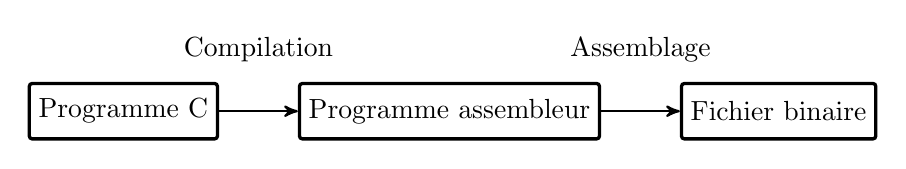
\begin{tikzpicture}[->,scale=1,>=stealth',thick]
\node[state] (PC) {Programme C};
\node[state, right=1.0cm of PC] (ASM) {Programme assembleur};
\node[state, right=1.0cm of ASM] (BIN) {Fichier binaire};

% \draw [-] (PC) -- (BIN) {Compilation};
\draw (PC) -- node[above=0.5cm]{Compilation} (ASM);
\draw (ASM) -- node[above=0.5cm]{Assemblage} (BIN);
\end{tikzpicture}}
\end{center}
\pause

\begin{block}{Code assembleur}
\begin{lstlisting}[language={[x86masm]Assembler}, style=verbo, escapechar=~,aboveskip=0pt,belowskip=0pt]
msg     db      "Hello, world", 0xa

mov     eax, 4 
mov     ebx, 1 
mov     ecx, msg 
mov	edx, len 
int     0x80        ; ~Appel système (Write)~
\end{lstlisting}
\end{block}
\end{frame}

\begin{frame}{Binaires et désassemblage}
\begin{center}
\scalebox{1}{
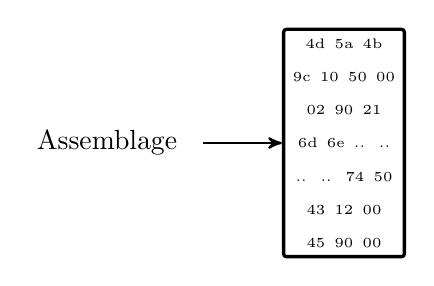
\begin{tikzpicture}[->,scale=1,>=stealth',thick,every text node part/.style={align=center}]
\node[state,draw=none] (PC) {};
% \node[state, right=1.0cm of PC] (ASM) {\begin{tiny} AB\\BA \end{tiny}};
\node[state, right=1.0cm of PC,text width=1.3cm] (ASM) {\tiny 4d 5a 4b 9c 10 50 00 02 90 21 6d 6e .. .. .. .. 74 50 43 12 00 45 90 00};
% \node[state, right=1.0cm of ASM] (BIN) {Fichier binaire};
% \draw [-] (PC) -- (BIN) {Compilation};
\draw (PC) -- node[left=0.7cm]{Assemblage} (ASM);
% \draw (ASM) -- node[above=0.5cm]{Assemblage} (BIN);
\end{tikzpicture}}
\end{center}

% \begin{tabular}[b]{|l|}
% \hline
% Entêtes\\
% \hline
% Sections\\
% ~~~~.text\\
% \hline
% ~~~~.data\\
% \hline
% ~~~~...\\
% \hline
% \end{tabular}
Désassemblage :
\begin{itemize}
 \item Opération inverse de l'assemblage
 \item Difficile de séparer les données du code
\end{itemize}

\begin{defi}
 Le désassemblage parfait d'un programme binaire est la donnée de l'ensemble de ses instructions atteignables.
\end{defi}
Il s'agit d'un problème indécidable.
\end{frame}

\begin{frame}{Graphe de flot de contrôle}
\begin{center}
\only<1>{
\begin{table}
% \small
\begin{tabular}[b]{|l|l|l|}
\hline
Adresse & Octets & Instruction\\ 
\hline
 8048067  &  b8 00 00 00 00         &  mov    eax,0x0 \\
 804806c  &  eb 05                  &  jmp    0x8048073 \\
 804806e  &  b8 03 00 00 00         &  mov    eax,0x3 \\
 8048073  &  83 f8 00               &  cmp    eax,0x0 \\
 8048076  &  74 06                  &  je     0x804807e \\
 8048078  &  b8 01 00 00 00         &  mov    eax,0x1 \\
 804807d  &  c3                     &  ret     \\
 804807e  &  b8 02 00 00 00         &  mov    eax,0x2 \\
 8048083  &  c3                     &  ret     \\
\hline
\end{tabular}
\end{table}
}
\only<2>{
\begin{minipage}{.5\textwidth}
  \centering
  \begin{table}
%   \tiny
  \begin{tabular}[b]{|l|}
  \hline
  Instructions\\ 
  \hline
  mov    eax,0x0 \\
  jmp    0x8048073 \\
  mov    eax,0x3 \\
  cmp    eax,0x0 \\
  je     0x804807e \\
  mov    eax,0x1 \\
  ret     \\
  mov    eax,0x2 \\
  ret     \\
  \hline
  \end{tabular}
  \end{table}
\end{minipage}%
\begin{minipage}{.5\textwidth}
  \centering
  \includegraphics[width=1.0\textwidth]{supports/eax-cfg/eax2_cropped0.pdf}
\end{minipage}
}
\end{center}
\end{frame}

\begin{frame}{Objectifs}
Analyse de programmes binaires obscurcis
\begin{itemize}
 \item Désassemblage : séparation du code et des données
 \item Reconstruction du graphe de flot de contrôle (GFC)
\end{itemize}

Détection de programmes malveillants et analyse de similarités logicielles
\begin{itemize}
 \item Comparaison des graphes de flot de contrôle
 \item Formalisation et optimisation
\end{itemize}

\end{frame}

\section{Obscurcissement et désassemblage}
\subsection{Difficultés}

\begin{frame}{Stratégies de désassemblage, obscurcissement}
\begin{minipage}{.5\textwidth}
  \centering
  \begin{table}
%   \tiny
  \begin{tabular}[b]{|l|}
  \hline
  Instructions\\ 
  \hline
  mov    eax,0x0 \\
  jmp    0x8048073 \\
  mov    eax,0x3 \\
  cmp    eax,0x0 \\
  je     0x804807e \\
  mov    eax,0x1 \\
  ret     \\
  mov    eax,0x2 \\
  ret     \\
  \hline
  \end{tabular}
  \end{table}
\end{minipage}%
\begin{minipage}{.45\textwidth}
  \centering
  \includegraphics[width=1.0\textwidth]{supports/eax-cfg/eax2_cropped0.pdf}
\end{minipage}

Désassemblage linéaire :
\begin{itemize}
%  \item Parcourt la première instruction du binaire puis l'instruction à l'adresse suivante
 \item Ne suit par le flot des instructions
\end{itemize}

Désassemblage récursif :
\begin{itemize}
%  \item Parcourt le point d'entrée puis les instructions pouvant potentiellement la suivre à l'exécution
 \item Donne une sur-approximation des instructions potentiellement exécutées
\end{itemize}
\end{frame}


\begin{frame}{Obscurcissement}
\begin{itemize}
 \item Ensemble de techniques utilisées pour rendre un binaire plus difficile à comprendre, analyser et désassembler
 \item En pratique appliquées par un logiciel d'empaquetage
\end{itemize}

\begin{center}
\scalebox{0.95}{
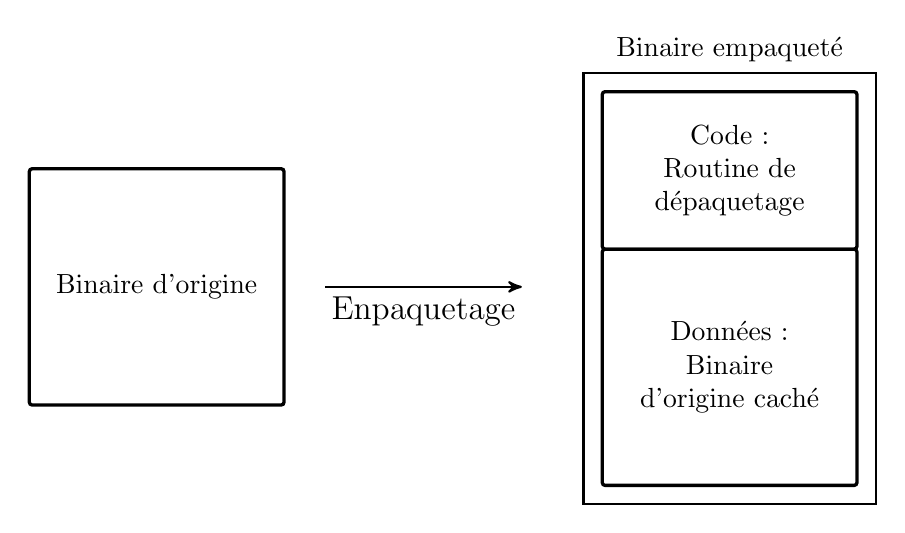
\begin{tikzpicture}[->,scale=1,>=stealth',thick]
\node[state, text width=3cm, minimum size=3cm] (BIN){Binaire d'origine};
\node[state, below right = -0.5cm and 4cm of BIN.east, text width=3cm, minimum size=3cm] (BINO){Données :\\Binaire d'origine caché};
\node[state, below = -2cm of BINO.north, text width=3cm, minimum size=2cm] (UNPACK){Code :\\Routine de dépaquetage};
% \draw ($(BIN.north west) + (-0.8, -0.1) $) -- node[left=0.3cm]{Point d'entrée} ($(BIN.north west) + (0, -0.1) $);
% \draw ($(UNPACK.north east) + (0.8, -0.1) $) -- node[right=0.3cm]{Point d'entrée} ($(UNPACK.north east) + (0, -0.1) $);
\draw ($(BIN.east) + (0.5, 0) $) -- node[below]{\large Enpaquetage} ($(BIN.east) + (3cm, 0) $);
\node [fit={($(UNPACK.north west) + (-0.1, 0.1)$) ($(BINO.south east) + (0.1, -0.1)$)}, draw, label=Binaire empaqueté] {};
\end{tikzpicture}
}
\end{center}
\end{frame}


\begin{frame}[fragile]{Chevauchement de code}
\begin{itemize}
 \item Technique d'obscurcissement statique
 \item Plusieurs instructions peuvent être codées sur des adresses qui se chevauchent
 \item Les techniques d'analyse font généralement l'hypothèse que ce n'est pas possible
\end{itemize}

\begin{block}{Exemple (\telock)}
Octets à désassembler : \texttt{eb ff c9 7f e6}
\begin{lstlisting}[language={[x86masm]Assembler}, escapechar=~]
01006e7d    eb ff           jmp +1
01006e7e       ff c9        dec ecx
01006e80    7f e6           jg 01006e68
\end{lstlisting}
\end{block}
\end{frame}

\begin{frame}[fragile]{Chevauchement de code : \underline{sémantique}}
\begin{block}{Exemple (\telock)}
Octets à désassembler : \texttt{eb ff c9 7f e6}
\begin{lstlisting}[language={[x86masm]Assembler}, escapechar=~]
01006e7d    eb ff           jmp +1
01006e7e       ff c9        dec ecx
01006e80    7f e6           jg 01006e68
\end{lstlisting}
\end{block}

\begin{center}
\begin{table}
\small
\begin{tabular}{|l|c|c|c|c|c|}
\hline
Adresses & 01006e7d & 01006e7e & 01006e7f & 01006e80 & 01006e81\\
\hline
Octets & eb & ff & c9 & 7f & e6\\
\hline
\Layer\ 1 & \multicolumn{2}{c|}{jmp +1} & \cnoir & \multicolumn{2}{c|}{jg 0x1006e68}\\
\hline
\Layer\ 2 & \cnoir & \multicolumn{2}{c|}{dec ecx} & \multicolumn{2}{c|}{\cnoir} \\
 \hline
% \\
\end{tabular}
\end{table}
\end{center}
\end{frame}



\begin{frame}[fragile]{Chevauchement de code : \underline{sémantique}}
\only<1-2>{
 \begin{defi}
 Une \layer\ de code $L$ est un ensemble d'instructions qui ne se chevauchent pas : $\forall D_1, D_2\in L,\ \mdc{I_1}\cap\mdc{I_2}=\emptyset$.
\label{def:layer}
\end{defi}

\begin{defi}
 Étant donné un ensemble d'instructions $E$, un découpage cohérent est un ensemble de \layers\ deux à deux disjointes et recouvrant l'ensemble des instructions de $E$.
\label{def:decoupage}
\end{defi}
}

\only<2>{
Quelle stratégie pour construire les couches de code ?
\begin{itemize}
 \item Couches linéaires
 \item Couches désassemblées par parcours
\end{itemize}

}
\end{frame}

\begin{frame}{Chevauchement de code : couches linéraires}
% Couches linéaires :
\begin{itemize}
 \item Une couche démarre à chaque adresse et consiste en un désassemblage linéaire
 \item Les couches redondantes sont éliminées
 \item La première couche correspond au désassemblage linéaire
 \item L'ensemble des couches est une généralisation du désassemblage linéaire
\end{itemize}

\begin{center}
\begin{tabular}{|l|c|c|c|c|c|}
\hline
Adresses & 01006e7d & 01006e7e & 01006e7f & 01006e80 & 01006e81\\
\hline
Octets & eb & ff & c9 & 7f & e6\\
\hline
\Layer\ 1 & \multicolumn{2}{c|}{jmp +1} & leave & \multicolumn{2}{|c|}{jg 0x1006e68}\\
\hline
\Layer\ 2 & \cnoir & \multicolumn{2}{c|}{dec ecx} & \multicolumn{2}{|c|}{jg 0x1006e68 \cgris} \\
\hline
\Layer\ 3 & \multicolumn{2}{c|}{\cnoir} & leave \cgris & \multicolumn{2}{|c|}{jg 0x1006e68 \cgris} \\
\hline
\Layer\ 4 & \multicolumn{3}{c|}{\cnoir} & \multicolumn{2}{|c|}{jg 0x1006e68 \cgris} \\
\hline
\Layer\ 5 & \multicolumn{4}{|c|}{\cnoir} & (invalide) \\
\hline
% \\
\end{tabular}
\end{center}
\end{frame}

\begin{frame}{Chevauchement de code : couches désassemblées par parcours}
% Couches linéaires :
\begin{itemize}
 \item Une couche démarre à chaque adresse et consiste en un désassemblage linéaire
 \item Les couches redondantes sont éliminées
 \item La première couche correspond au désassemblage linéaire
 \item L'ensemble des couches est une généralisation du désassemblage linéaire
\end{itemize}

\begin{center}
\begin{tabular}{|l|c|c|c|c|c|}
\hline
Adresses & 01006e7d & 01006e7e & 01006e7f & 01006e80 & 01006e81\\
\hline
Octets & eb & ff & c9 & 7f & e6\\
\hline
\Layer\ 1 & \multicolumn{2}{c|}{jmp +1} & leave & \multicolumn{2}{|c|}{jg 0x1006e68}\\
\hline
\Layer\ 2 & \cnoir & \multicolumn{2}{c|}{dec ecx} & \multicolumn{2}{|c|}{jg 0x1006e68 \cgris} \\
\hline
\Layer\ 3 & \multicolumn{2}{c|}{\cnoir} & leave \cgris & \multicolumn{2}{|c|}{jg 0x1006e68 \cgris} \\
\hline
\Layer\ 4 & \multicolumn{3}{c|}{\cnoir} & \multicolumn{2}{|c|}{jg 0x1006e68 \cgris} \\
\hline
\Layer\ 5 & \multicolumn{4}{|c|}{\cnoir} & (invalide) \\
\hline
% \\
\end{tabular}
\end{center}
\end{frame}

\begin{frame}{Auto-modification}

\end{frame}

\subsection{Sémantiques}
\begin{frame}{Traitement de l'auto-modification}

\end{frame}

\begin{frame}{Traitement du chevauchement de code (original)}

\end{frame}

\subsection{Notre approche}
\begin{frame}{Graphe de flot de contrôle parfait}

\end{frame}

\begin{frame}{Graphe de flot de contrôle paramêtré}

\end{frame}

\begin{frame}{Codisasm}

\end{frame}

\section{Algorithmes de comparaison}
\subsection{Analyse morphologique}
\begin{frame}{Détection de similarités logicielles}

\end{frame}

\subsection{Formalisation et simplification}
\begin{frame}{Isomorphisme appliqué aux graphes de flot}

\end{frame}

\subsection{Algorithmes et implémentation}
\begin{frame}{Algorithme par parcours}

\end{frame}

\begin{frame}{SIDT}

\end{frame}

\begin{frame}{Comparaison des performances}

\end{frame}

\begin{frame}{Implémentations}

\end{frame}

\section{Exemples d'application}

\begin{frame}{OpenSSL / Waledac}

\end{frame}

\begin{frame}{Duqu / Stuxnet}

\end{frame}

\section{Conclusion}

\begin{frame}{Conclusion}
\begin{itemize}
\item Analyse et désassemblage de programmes binaires obscurcis
\item Détection de similarités par comparaison des graphes de flot de contrôle
\item Application sur quelques cas de programmes malveillants
\end{itemize}
% Still to be done :
\pause
\begin{itemize}
\item Merci
\item Des questions ? (aurelien@athierry.fr)
% \item Loop detection and comparison for dynamic analysis
% \item Better reductions to detect through obfuscation
% \item Smoother UI for the IDA plugin
\end{itemize}
\end{frame}



\makeatletter
  \immediate\write\@mainaux{\string\gdef\string\inserttotalframenumbernew{\insertframenumber}}
\makeatother
\appendix


% \begin{frame}[allowframebreaks]
% \section*{}
% {
% \frametitle{Références}
% \bibliography{../rapportbib}
% \bibliographystyle{alpha}
% }
% \end{frame}

% % suppléments :
% \begin{frame}{More}
% \end{frame}




\end{document}
